\section{Experimental Evaluation: comparing provenances}
\label{sec:experiments}
To understand the tradeoff between these distribution strategies, we performed three sets of experiments using queries over GtoPdb.  The first set of experiments used real queries extracted from citations to GtoPdb published in the British Journal of Pharmacology.  
The second set uses different sets of synthetically produced provenance polynomials, corresponding to more complex queries, apt to highlight the differences between the DS.
In the third set of experiments we compare the differences between traditional citations and credit in rewarding data curators. 

\subsection{Real-world queries}
\label{sec:real_world_queries}

\begin{figure}[t]
  \includegraphics[width=1\textwidth]{figures/paper_based}
  \caption{Comparison of three DS on the same table \texttt{family} using the distribution given by the queries retrieved from papers.}
  \label{figure:comparison_on_papers}
\end{figure}


We evaluate the proposed distribution strategies on GtoPdb, and in particular we focus on target families, all of those are described in pages of the GtoPdb website. 
There are eight family types: \emph{GPCR}, \emph{Ion channels}, \emph{NHRs}, \emph{Kinases}, \emph{Catalytic receptors}, \emph{Transporters}, \emph{Enzymes} and \emph{Other protein targets}.  

When a paper uses data from GtoPdb, it can cite the full database, the webpage of interest, or a subset of data extracted with a query. 
We consider as sources of citations the papers published in the British Journal of Pharmacology (BJP)~\footnote{\url{https://bpspubs.onlinelibrary.wiley.com}}, since each time they cite a webpage from GtoPdb, they report the URL of that page. From that URL it is possible to reverse-engineer the queries that are used to obtain the data contained in the pages. 
In particular, we considered all the $889$ papers in BJCP citing \citep{iuphar2018} as of October 2020. \citep{iuphar2018} is a data journal that describes the structure and evolution of GtoPdb. ERach two years the GtoPdb consortium releases such a journal to describe the evolution of the databases.
At the time of writing, this paper received more than $1200$ citations. 

The queries that we inferred are the ones building the information that constitutes a target family webpage are depicted in Figure \ref{figure:family_structure} (with the exception of the section References). 
In the figure, we can see how the structure of one family, ``Adenosine receptors'', is mapped into several queries to obtain the information to build the corresponding webpage. 
In GtoPdb, all target family pages share a similar structure (the only differences is that certain sections, such as ``contributors'' or ``further readings'', may be absent).
The same queries can therefore be used to build all the target family pages by simply changing the family id used in the query (which, in the example of Figure \ref{figure:family_structure}, is 3). All these queries are SPJ. 
A total of more than $12K$ different queries were built in this way\footnote{For reproducibility purposes, the code we used for our experiments and all the produced queries can be found at the following link: \url{https://bitbucket.org/dennis_dosso/credit_distribution_project}.}.
We assumed that each tuple in the output of each of these queries carries credit 1.

Figure \ref{figure:comparison_on_papers} shows the heat-maps obtained by the distribution of credit performed by the three different DS on the GtoPdb table \texttt{family}.
\texttt{family} is a table describing the characteristics and basic information of the receptor families and, as can be seen in Figure \ref{figure:family_structure}, it is often used in join with other tables in the queries that build a webpage.

It is immediately evident that the result of the distribution is the same with the three strategies. The same effect is also obtained in the other tables of the database used by the queries shown in Figure \ref{figure:family_structure}. 

Why is that? 
It is the case that the conditions in which we produced this experiment are quite peculiar. The queries that we used share similar characteristics. They are all SPJ queries, each of them utilizes each table only once in the join condition (there are no self-joins), and all the joins are made using key attributes. 
In this particular condition, each tuple of the output presents: (i) a how-provenance that is a single monomial with coefficient $1$ and exponent $1$ in each variable; (ii) a why-provenance that is composed by only one witness; (iii) a lineage that coincides with the only witness in the witness basis.
It is easy to see how, given these queries, the three distributions act in the same way.
The credit is always uniformly distributed among the tuples appearing in each provenance. 

To better clarify what is happening, let us consider one of the types of queries used to build the output webpage, as shown in Figure \ref{figure:family_structure}:

\vspace{2mm}
{\footnotesize
\begin{adjustwidth}{25pt}{5pt}
	\begin{verbatim}
	Q3: SELECT c.first_names, c.surname
	FROM contributor2family AS cf JOIN contributor AS c ON 
	cf.contributor_id = c.contributor_id 
	WHERE f.family_id = 3
\end{verbatim}
\end{adjustwidth}
}
\vspace{2mm}

\texttt{Q3} returns a series of $10$ tuples from the version of GtoPdb we considered. 
The first tuple produced by this query, \texttt{<Bertil B., Fredholm>}, that has $c_{939} \cdot c2f_{496}$ as provenance polynomial.
$c_{939}$ represents the provenance token of a tuple in \texttt{contributor}, the same for $c2f_{496}$ in table \texttt{contributor2family}. 
It is easy to see that the why-provenance of this tuple is $\{\{c_{939}, cf_{496} \}\}$ and its lineage is $\{c_{939}, c2f_{496} \}$.
Therefore, the credit assigned to these tuples is $1/2$ using all three DS.
This actually happens for each tuple of the output of each query of GtoPdb, thus making the distributions equivalent with respect to their output.

This is not always the case with general queries and other databases. As we showed in the examples in the previous section, when two or more tuples are merged by the effect of a projection or union, we see sensible differences between the three distribution strategies. %These are represented as multiple witnesses and multiple monomials. 

\begin{comment}
	
To give an example of how the CDS can differ from one another in their behavior, let us consider a different query:

\vspace{2mm}
{\footnotesize
\begin{adjustwidth}{25pt}{5pt}
	\begin{verbatim}
	Q4: SELECT f.name AS name
	FROM family AS F JOIN
	(SELECT DISTINCT f.family_id, f.name
	FROM "family" AS f JOIN contributor2family AS cf ON 
	f.family_id = cf.family_id 
	JOIN contributor c ON 
	cf.contributor_id = c.contributor_id 
	WHERE c.country = 'UK') AS R 
	ON F.name = R.name
\end{verbatim}
\end{adjustwidth}
}
\vspace{2mm}

Here the innermost query retrieves all the names and ids of the families written by an author from the UK producing a relation called $R$. This relation is then joined with the table \texttt{family} on the attribute \texttt{name}. 

One output tuple of this query is \texttt{<Histamine receptors>}, that has the following provenance polynomial:

{\footnotesize
\[
\begin{array}{c}
	f_{625}(f_{625} c2f_{656} c_{184} + f_{625} c2f_{113} c_{180} + f_{625} c2f_{283} c_{198} +\\ 
	+ f_{625} c2f_{550} c_{865} + f_{625} c2f_{573} c_{101} + f_{625} c2f_{95} c_{109} )
\end{array}
\]
}

As already discussed, the different monomials represent possible \emph{alternatives} of combinations of tuples that produce the considered output tuple. 
Tuple $f_{625}$ is used multiple times with different joins, thus it appears in each monomial. 
The last join, performed in the outmost query, is responsible for the final multiplication of $f_{625}$ with the rest of the polynomial between parenthesis.

From this polynomial we compute the why-provenance as a set of six different witnesses:

{\footnotesize
\[
\begin{array}{c}
\{\{ f_{625}, c2f_{656}, c_{184} \}, \{ f_{625}, c2f_{113}, c_{180} \} 
\{ f_{625}, c2f_{283}, c_{198} \}, \\ \{ f_{625}, c2f_{550}, c_{865} \},
 \{ f_{625}, c2f_{573}, c_{101}\} , \{f_{625}, c2f_{95}, c_{109} \}\}	\\
\end{array}
\]
}

And corresponding lineage:
{\footnotesize
\[
\begin{array}{c}
	\{ f_{625}, c2f_{656}, c_{184}, c2f_{113}, c_{180}, 
  c2f_{283}, c_{198}, c2f_{550}, c_{865}, 
  c2f_{573}, c_{101}, c2f_{95}, c_{109}\}
\end{array}
\]
}

\begin{figure}[tb]
  \includegraphics[width=1\textwidth]{figures/synthetic_queries}
  \caption{Comparison of three DS on the same table \texttt{family} after the distribution of the credit connected to query \texttt{Q4}.}
  \label{figure:comparison_on_synthetic_query_1}
\end{figure}

This was only one tuple among the $86$ obtained from this query. If we assign credit $1$ to all these tuples and distribute it with the different strategies, we obtain the result shown in Figure \ref{figure:comparison_on_synthetic_query_1} for the table \texttt{contributor}.
At first sight, it may appear that the three distributions produce the same result. This is only partially true: the heat maps appear equal, but the absolute values assigned to each tuple are different. 
This is more evident if we look at the legend of each heat-map, where the maximum quantity of credit is different for each distribution. The one performed through lineage is around $1.8$, the why-provenance's one is around $1.4$, and the one based on how-provenance is around $1.1$. 

To understand what is happening with this query in this specific table, consider the output tuple \texttt{<Histamine receptors>} and its provenances, as discussed above.
Let us focus on its lineage. There are a total of six authors for this family and $13$ tuples in total in the lineage. 
Thus, using the lineage-based DS, each tuple belonging to the \texttt{contributor} table (i.e. $c_{184}, c_{180}, c_{198}, c_{865}, c_{101}, c_{109}$) receives credit equal to $1/13$.
Tuple $f_{625}$ too receives a portion of credit equal to $1/13$.

Let us consider now why-provenance. Tuple $f_{625}$ appears six times in six different witnesses composed of $3$ elements each. From each witness it receives a portion of credit equal to $1/18$, thus its total credit is $1/3$.
On the other hand, all the authors appear only once in each witness, thus each of them receives credit $1/18$. 
In this case, why-provenance is recognizing more credit to tuple $f_{625}$, since it appears in each witness. The consequence is that this distribution is equally \emph{subtracting} credit from the other tuples in the witnesses and giving it to $f_{625}$. 
In Figure \ref{figure:comparison_on_synthetic_query_1} we are only looking at table \texttt{contributor}. 
This same effect is reproduced for each tuple of the output of query \texttt{Q4}, thus the \emph{absolute} credit values on the tuples vary depending on the deployed strategy. 
What happens is that the tuples in table \texttt{contributor} receive less credit than the one received using lineage, but in the same proportions. The heat map appears thus equal to the one obtained with lineage.
This same effect is also present with the how-provenance-based CDS. In this case, tuple $f_{625}$ is rewarded even more, since it appears with an exponent 2 in each monomial, thus attracting even more credit. 

This is also why when we look at the legend for each part of Figure \ref{figure:comparison_on_synthetic_query_1}, the maximum value reached with the lineage-based DS is higher than the one reached with the why-provenance-based DS, which in turn is higher than the one obtained with the how-provenance. This is because the different strategies reward less and less the tuples of table \texttt{contributor} and more the ones in table \texttt{family}. 

This clearly shows the ability of the different strategies to adapt to situations. All three of them can highlight the relevant tuples in the table. However, they differ in the way they reward the tuples. 
Depending on the task, one provenance can be preferred to the other. 
If the only interest is to highlight the relevant tuples, lineage is sufficient. 
If the interest is also to reward more the tuples that are fundamental to the output, one can also choose why- or how-provenance, knowing that how-provenance rewards even more than why-provenance the relevant tuples that are indispensable for the output.  

\end{comment}


\subsection{Synthetic queries}

\begin{figure}[tb]
  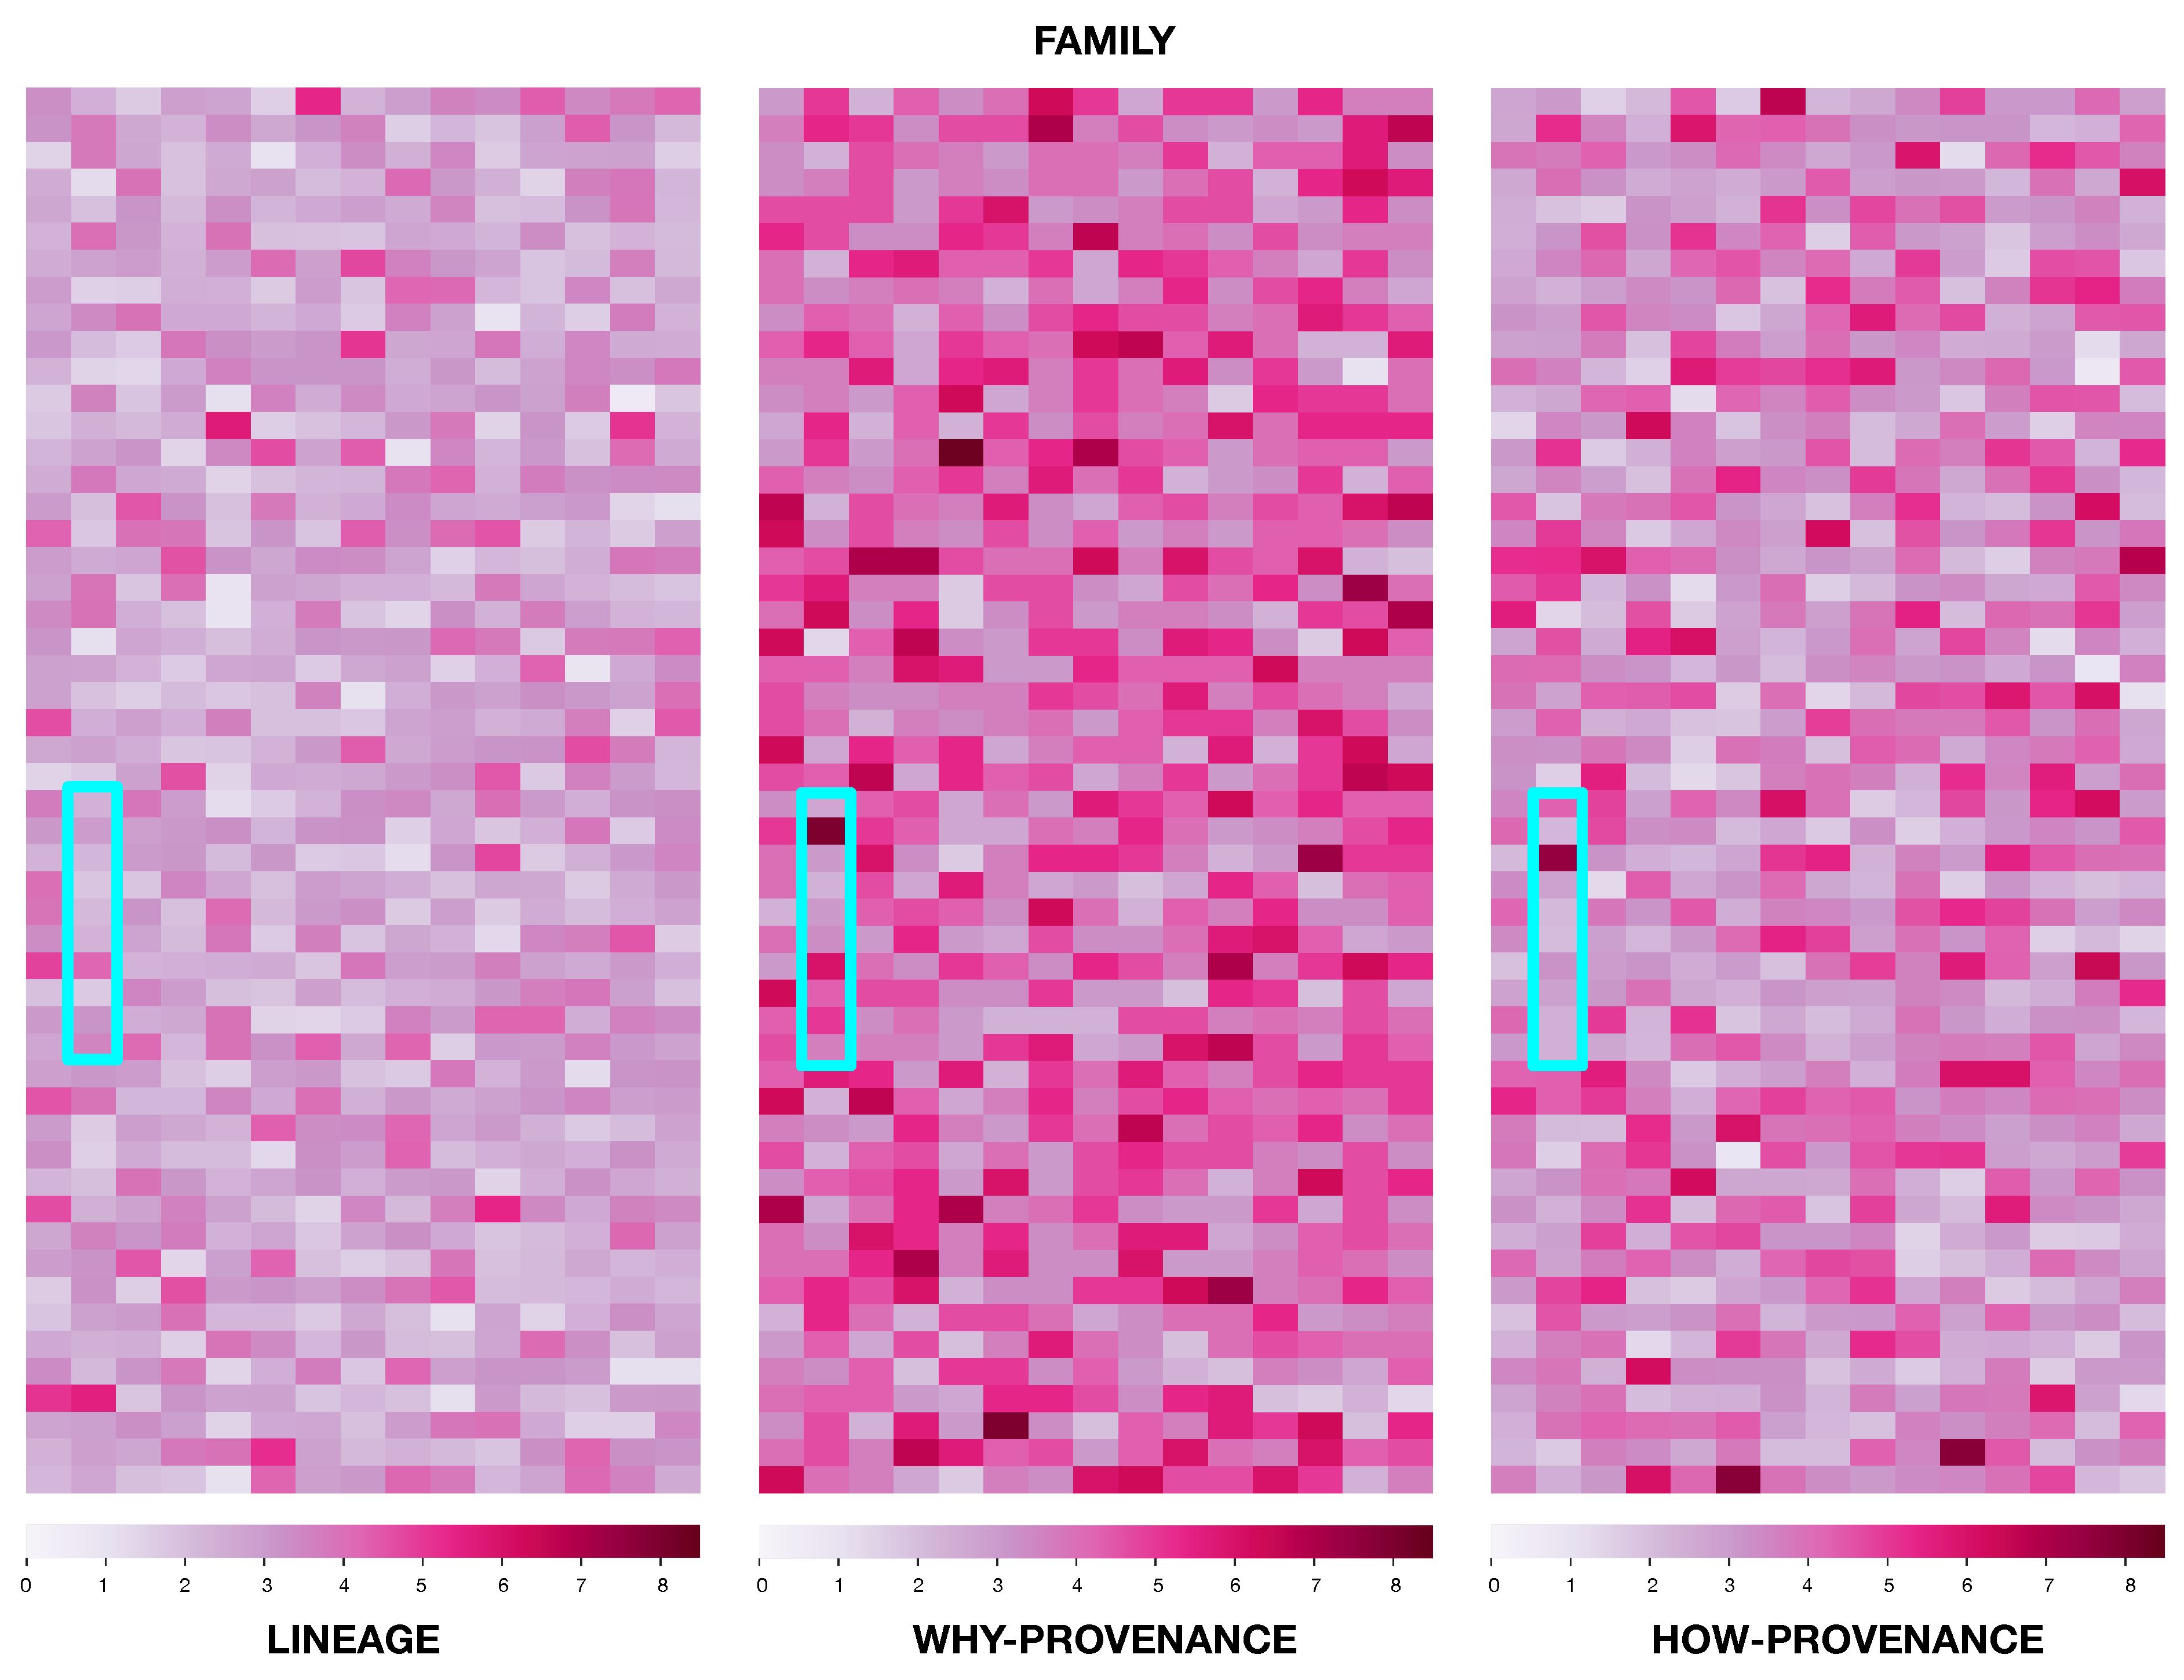
\includegraphics[width=1\textwidth]{figures/synthetic_polynomials}
  \caption{Comparison of three DS on the same table \texttt{family} after the distribution computed using 10K synthetic and randomly generated provenance polynomials. The tuples in the blue rectangles are used as example in the discussion connected to Figure \ref{fig:comparison}.}
  \label{figure:comparison_on_synthetic_polynomials_2}
\end{figure}

To show how the three DS can actually behave differently, let us consider another case shown in Figure \ref{figure:comparison_on_synthetic_polynomials_2}. 


The figure reports a distribution of credit performed on the table \texttt{family} through the generation of 10K \emph{synthetic} polynomials. 
We randomly generated provenance polynomials that might be the how-provenance of randomly generated synthetic queries, using the three GtoPdb tables \texttt{family}, \texttt{contributor2family}, and \texttt{contributor}. 
An example of such synthetic polynomial is:
{\footnotesize
\[
3 f_1^3 c2f_1^2 c_1^2 + 2 f_1 c2f_2^3 c_2^3 + 4 f_5 c2f_{17}^4 c_{18}^3
\] }

As can be seen, we made sure to also include coefficients and exponents that differ from $1$.
Its corresponding why-provenance is: 
{\footnotesize
\[
\{ \{f_1, c2f_1, c_1\}, \{f_1, c2f_2, cf_2\}, \{ f_5, c2f_{17}, c_{18}\} \}
\] 
}

its lineage is: 
{\footnotesize
\[
\{f_1, f_5, c2f_1, c_1, c2f_1, c2f_2, c2f_{17}, c_1, c_2, c_{18} \}
\]
 }
 
These types of polynomials are not impossible to obtain in real life, since they can be obtained by nested queries with join and union operations that use multiple times the same tuples (thus the presence of exponents bigger than $1$) and the same combination of operations more than once (thus the presence of coefficients for monomials bigger than $1$). 
We randomly generated a set of $10$K such polynomials. 

Using how-provenance, this is the distribution obtained from the example polynomial we are considering:
{\footnotesize
\[
f_1 = \frac{59}{315}, f_5 = \frac{1}{18}, c2f_1 = \frac{2}{21}, c2f_2 = \frac{2}{15}, 
c2f_{17}=\frac{2}{9} , c_1 = \frac{2}{21}, c_2 = \frac{2}{15}, c_{17} = \frac{1}{6} 
\]
}

Using why-provenance, this is the output:
{\footnotesize
\[
f_1 = \frac{2}{9}, f_5 = \frac{1}{9}, c2f_1 = \frac{1}{9}, c2f_2 = \frac{1}{9}, 
c2f_{17}=\frac{1}{9} , c_1 = \frac{1}{9}, c_2 = \frac{1}{9}, c_{17} = \frac{1}{9} 
\]
}


Finally, with lineage, this is the distribution:
{\footnotesize
\[
f_1 = \frac{1}{8}, f_5 = \frac{1}{8}, c2f_1 = \frac{1}{8}, c2f_2 = \frac{1}{8}, 
c2f_{17}=\frac{1}{8} , c_1 = \frac{1}{8}, c_2 = \frac{1}{8}, c_{17} = \frac{1}{8} 
\]
}

To highlight how the distributions behave differently with these polynomials, consider tuple $f_5$.
$f_5$ receives the highest quantity of credit when we use the lineage-based distribution. Why-provenance and how-provenance reduce its quantity of credit since more information is available for the computation and the algorithms weigh less and less its role. 

Generally speaking, the more complex the distribution, the more polarized the credit is toward the tuples that are used more frequently or with a higher impact in the production of the output tuple. 

Going back to Figure \ref{figure:comparison_on_synthetic_polynomials_2}, it is thus possible to observe empirically how the three provenances behaved differently. We put the maximum value for the heat-maps around $8.33$, since that is the highest value reached by a tuple in all three distributions. 
We note that lineage is the provenance that gives less credit to the tuples of the \texttt{family} table. This is due to the fact that the DS equally distributes the credit to all the tuples appearing in the lineage. Since other two tables are used by these queries, the credit is also given to the tuples of those tables. 

Moving to the heat-map reporting the distribution performed by the DS based on why-provenance, we see that this time more credit is given overall to the tuples of the table. Actually, this DS is the one that distributes more credit to \texttt{family} among the three strategies. 
This is due to the fact that the DS based on why-provenance also takes into account the different ways in which a tuple is used, e.g. in different joins. If the same tuple is present in more than one witness, it is more probable that it will attract more credit, ``stealing'' it from the other tuples in the witness basis. In this case, \texttt{family} was able to attract more credit, taking it from the other two tables, due to the role of its tuples in the queries that were executed.

Considering now the heat-map produced by the DS based onhow-provenance, we see how, although it presents more credit in its tuples that the one present in the lineage heat-map, it does not reaches the levels of the why-provenance heat-map.
This is due to the fact that this DS is even more sophisticated, weighting even more than the previous DS the role of tuples in the production of the output. 
The result is a distribution that still rewards the tuples of this table more than lineage, but not in the same measure as the DS based on why-provenance, since the other tuples in the other tables are able to attract more credit due to their roles in the queries. 

%%%%%%%%%%%%%%%%%%

To show how the DS based on different provenances may actually differ in their behavior also through the course of time, let us consider Figure \ref{fig:comparison}.

\begin{figure}[t]
  \includegraphics[width=\textwidth]{figures/comparison_2}
  \caption{Comparison of the distribution of credit performed by the three DSs on a subset of 10 tuples taken from table \texttt{family} simulating the passing of time. The number on top of each group of heat-maps represent the number of queries computed.}
  \label{fig:comparison}
\end{figure}

In this figure we report four groups of heat-maps. Each group presents three maps obtained by selecting the same ten tuples from the GtoPdb \texttt{family} table after an incremental distribution of credit (the tuples of ranks ranging from 79 to 89). These are the same tuples highlighted in the blue boxes in Figure \ref{figure:comparison_on_synthetic_polynomials_2}.  In particular, the four groups represents ``snapshots'' taken during an incremental accumulation of credit on the database, at different moments chosen when a certain number of executed queries is reached (specifically, 1K, 2K, 5K and 10K).
Figure \ref{figure:comparison_on_synthetic_polynomials_2} represents the end of the process. 

In this way we are simulating the passing of time on a database where credit distribution is performed. Each group of heat-maps can be thought as a snapshot of that set of tuples at a certain moment, after a certain amount of queries are executed. 
The queries utilized are the same of the experiment of the previous section. The range of credit in each map goes from 0 (no credit) to 6 (maximum quantity of credit reached on a tuple at the ``snapshot'' reached at 10K queries).

Focusing on the 1K and 2K groups, we see that the three DS do not behave very differently. The tuples highlighted by the three are almost the same. There are still small differences, in particular in tuple 5.

The first interesting interesting differences appear at 5K queries. In particular, we note how tuple 7 is rewarded poorly by the DS based on lineage, while it is rewarded more by why-provenance-based DS and most of all by the DS based on how-provenance. This is due to the fact that tuples 7 appears in a relative low number of lineages, but its role is critical to these queries, thus the other DS reward it more.
On the other hand, a tuple as 5 is rewarded by the DS based on lineage and why-provenance, and less by how-provenance. This means that, although tuple 5 appears in many queries and it is used in different combinations, its exponents in the provenance polynomials where it appears must be low, therefore giving it low credit with how-provenance.
It is also interesting to note how certain tuples, like 1, that up until 2K queries presented the highest values of credit, are now surpassed by other tuples like 2. This shows how credit is able, during the passage of time, to keep track of the ``hotspots'' in a database. The presence of new queries and new credit distribute can change the hotspots in a table, showing how the interests of the research community may change during time. 

Finally, the highest differences are shown in the 10K group. In this case, we see a situation similar to the one already seen with the case of 5K queries. Certain tuples, like 8 or 10, receive more credit with why-provenance and how-provenance, rather than with lineage. This is still due to the important role of the tuple in the queries where it appears. 

From this progression we see how, given the peculiar synthetic provenance polynomials that we presented, it is actually possible to see the differences between the three distribution. These differences become more and more evident with the passing of time, i.e. the more credit is distributed to the tuples. 

Therefore, although all the three DS considered here are effective in distributing credit, they actually behave differently. 
The DS based on lineage is sufficient when a user only wants to highlight the tuples of the database that are used by a query (and not only visualized in the output). However, it distributes the credit equally to the tuples of the lineage, therefore losing information on the role of the tuples in the production of the output. 

For this, a user may want (depending on the nature of the queries) to use DS based on why-provenance and how-provenance. The two are more sensitive than the DS based on lineage (and the DS based on how-provenance is more sensible than the one based on why-provenance). 
Therefore, using these DS, it is possible to change the distribution of credit to the tuple, rewarding more the tuples that have a more important role in the generation of the output. These two DS can therefore be preferred when the aim of the user is to find ``hotspots'' in the database based on the role of the tuples. 

In particular, the DS based on why-provenance rewards more the tuples that are used in different ways by queries (i.e. are members of more witnesses). The DS based on how-provenance also takes into consideration how many times a tuple is used, adding even more sensibility to the distribution. 
One may choose one other the other depending what are the aspects he wants to highlight in the data.

%%%%%%%%

\subsection{Credit vs Citations}

\begin{figure}[]
\centering
  \includegraphics[width=1\textwidth]{figures/2_radars}
  \caption{Radars presenting the top 20 authors citation-wise and credit wise, together with their (normalized between 0 and 1) values of citations and credit.}
  \label{figure:2_radars}
\end{figure}

For our last set of experiments, we confront traditional citations and credit, to see if they differ in their behaviour in the case if rewarding the curators of data.
Consider first Figure \ref{figure:2_radars}, where we report two radar plots.
The first plot presents the top 20 author (we identify the authors with their ID instead of their name), ordered based on the normalized value of citations distributed by the queries taken from the papers published in BJP as described in Section \ref{sec:real_world_queries}, together with their normalized value of credit. 
An author transitively receives credit from the data of which he or she is the curator. That is, the credit assigned to data is then split equally to the authors of those tuples. 
As we show in Section \ref{sec:real_world_queries}, there is no difference for these queries in the distribution of credit between the three DS, thus these values are equal for the three distributions.  
The second plot is similar to the first one, but the authors are ordered based on the received credit. 

As we see, the quantity of credit does not follow the quantity of citations, i.e. it is not true that an author that presents the highest number of citations also has the highest value of credit. 
As shown in Figure \ref{figure:2_radars}.b, the authors with the highest value of credit do not also have the highest number of citations. 
This means that there are citations that are much more ``valueble'' for an author in terms of credit. This is due to the fact that the quantity of credit assigned by these citations is very high, i.e. the impact of those cited data is high. 

This shows how credit is able to reward authors that are cited less than others but, nonetheless, have a high impact on the research community. 


\begin{figure}[t]
\centering
  \includegraphics[width=1\textwidth]{figures/3_radars}
  \caption{Radars presenting 20 authors ordered citation-wise and credit-wise, together with their (normalized between 0 and 1) values of citations and credit, through the execution of different numbers of polynomials (100, 1K, and 10K). The radar plots ordered by credit consider the credit assigned by the DS based on how-provenance.}
  \label{figure:3_radars}
\end{figure}

Consider now Figure \ref{figure:3_radars}.
In this case, we produced $100$, $1K$, and $10K$ synthetic polynomials and we distributed credit and assigned citations through them. Since these polynomials correspond to queries whose authors are not easily identifiable, we created $20$ ``synthetic'' authors, and we randomly assigned one author to each tuple in the database. The authors receive ``blocks'' of consecutive tuples, with each block of the size varying between $10$ and $40$. 
Every time a tuple was used in a provenance polynomial, we assigned one citation to the author corresponding to the tuple.  The same author also receives the three different credits assigned to the tuple at the end of the distribution process using the three DS.

The three radar plots in the upper row presents 20 authors are sorted based on the normalized number of received citations, together with the corresponding normalized quantities of credits assigned using the 3 different strategies.
The ones in the bottom row present the authors ordered based on the quantity of credit assigned by the DS based on how-provenance.
In this way we can see the behavior of the different DS in rewarding the authors with the highest levels of citations. 
Given the synthetic nature of these queries, the correlation between the number of citations and the quantity of credit assigned to the authors appears to be a much stronger with respect to the case with the real-world queries.

Nonetheless, it is possible to note that credit still behaves differently,. In particular we still see that certain authors that are not in the top 10 positions citation-wise are still rewarded with high quantities of credit, showing their importance with respect to their impact. 
Interestingly, scaling up to $1K$ and $10K$ polynomials, it appears that the distribution performed via why-provenance and how-provenance become equivalent for the authors. We can note that, although not exactly equal, the values of credit assigned to the authors by those DS become quite similar with these higher quantities of polynomials. 

\subsection{Execution times}

\begin{table}[hbt]
\centering
  \begin{tabular}{| l |c | c | c | c ||}
  \hline
    \# of polynomials  & lineage & why-prov. & how-prov. \\
    \hline
    100 & 226.6 ms & 192.0 ms & 185.5 ms \\
    200 & 431.2 ms & 392.2 ms & 403.2 ms \\
    500 & 1.013 s  & 934.2 ms & 881.8 ms \\ 
    1K  & 2.041 s  & 1.934 s  & 1.744 s  \\
    2K  & 3.773 s  & 3.491 s  & 3.510 s  \\
    5K  & 8.992 s  & 8.653 s  & 8.889 s  \\
    10K & 17.10 s  & 16.84 s  & 16.84 s  \\
    20K & 34.59 s  & 35.30 s  & 39.70 s \\
    100K & 3.289 min & 3.442 min & 3.652 min \\
    1M  & 35.91 min & 34.87 min & 37.91 min \\
    \hline
  \end{tabular}
  \caption{The times required to perform the three DS for different number of synthetic polynomials.}
  \label{table:times}
\end{table}

In Table \ref{table:difference_result} we report the time required to compute the distribution using the DS based on the three provenances as described above. As we see, the execution time grows linearly with the number of polynomials that are submitted to the system. With high values of polynomials (1M), the time required by the DS based on lineage and why-provenance is lower than the time required by the DS based on how-provenance, due to the bigger number of operations the last DS requires during the computations of the portions of credit to assign to the different tuples. 
We note that, since we created these polynomials on-the-fly, these values do not include the time required to compute the provenances.
Therefore, limited to the time required to distribute credit, the three DS are equivalent in terms of performances. The first differences can be seen only with high number of polynomials, when lineage and why-provenance may be preferred if there are no requirements to assign credit with the strategy implemented by the how-provenance-based DS.

All the experiments were carried on a MacBook Pro 13-inch, 2019 with 2.4 GHz processor Intel Core i5 quad-core, 8 GB of memory at 2133 MHz with code written in Java and the support of a PostgreSQL database. 


%\subsection{Discussion}
%
%In the previous sections we showed, through the use of different experiments, the behavior of credit and its distribution with the use of different DS. 
%It appeared that, in the case of SPJ queries, the three distributions behave in the same way on GtoPdb. 
%
%Using synthetic polynomials, we showed how the three DS actually behave differently, in particular with the passage of time, i.e. when more and more polynomials are processed. 
%The three DS are all effective ways to distribute credit, and there is not one distribution that is preferable to the other all the time. It all depends on the needs of the users. 
%
%Lineage is to be preferred when users only want to find tuples that are used in a database by queries applied to this database. With the accumulation of credit coming from many queries, the DS based on lineage is also able to create ``hotspots'' among the tuples of the relational database.
%However, lineage rewards equally the tuples used by a query.
% 
%Why-provenance is more versatile when users also want to consider how many ways a tuple is used; thus, in a way, its \emph{versatility} inside the queries that used it.
%Finally, how-provenance also counts how many times a tuple is used, its \emph{frequency} in the computation of a query. 